\documentclass[12pt]{article}
\usepackage{a4}
\usepackage[english]{babel}
\setlength{\parindent}{0.35cm}
\pagestyle{headings}
\usepackage{graphicx}
\usepackage{grffile}
%Multiple picture in one figure
%\usepackage{subfigure}
\usepackage{subfig}
\usepackage[utf8]{inputenc}
\usepackage{listings}
\usepackage{color}
\usepackage{wrapfig}
%Floating-Umgebungen
\usepackage{float}
%Math-Environment
\usepackage{amsmath}
\usepackage{amssymb}
%Better SI-Units
\usepackage{siunitx}
%Using Appendix
\usepackage[title]{appendix}
%Using URL
\usepackage[hidelinks]{hyperref}
%Using Colored Tables
\usepackage{colortbl}
\newcommand{\gray}{\rowcolor[gray]{.90}}
\usepackage{esvect}
% Use fancy tables
\usepackage{tabularx}
% Build fancy tables
\usepackage{booktabs}
%Configure geometry
\usepackage{geometry}
\geometry{
	a4paper,
	left=3cm,
	right=3cm,
	top=3cm,
	bottom = 3cm,
	}

\lstset{
	language=C++,
	basicstyle=\small\ttfamily,
	keywordstyle=\color{blue}\ttfamily,
	stringstyle=\color{red}\ttfamily,
	commentstyle=\color{green}\ttfamily,
	morecomment=[l][\color{magenta}]{\#},
}


\usepackage{amsthm}

\renewcommand\qedsymbol{$\blacksquare$}
\newtheorem{theorem}{Theorem}[section]

\begin{document}
	
	\title{
		\textbf{\huge{CSE 446: Machine Learning Winter 2018 }} \\[2cm]
		\LARGE{Assignment 2}\\[1cm]
	}
	\author{from \\ Lukas Nies \\ University of Washington}
	\date{02/01/18}
	\clearpage\maketitle\thispagestyle{empty}
	\newpage

	\tableofcontents
	\setcounter{page}{0}
	\newpage
	
	% To start with section 1 labeled as section 0
	\setcounter{section}{-1}
	

\section{Policies}

\subsection{List of Collaborators}

My collaborators were Edith Heiter (discussed Problem 2 and 4) and Julia Hess (discussed ?). The development of the answers though was completely independent and individually.

\subsection{List of Acknowledgments}

None.

\subsection{Policies}

I have read and understood these policies.

\section{Perceptron Exercise}

The evolution of the weight vector $w$ are shown in figure \ref{fig:1.1} after the data was observed so the weights were already updated. In the same figure the maximum margin is shown since the perceptron didn't maximize the margin after the training set.

\begin{figure}[b!]
	\centering
	\subfloat[Step One] {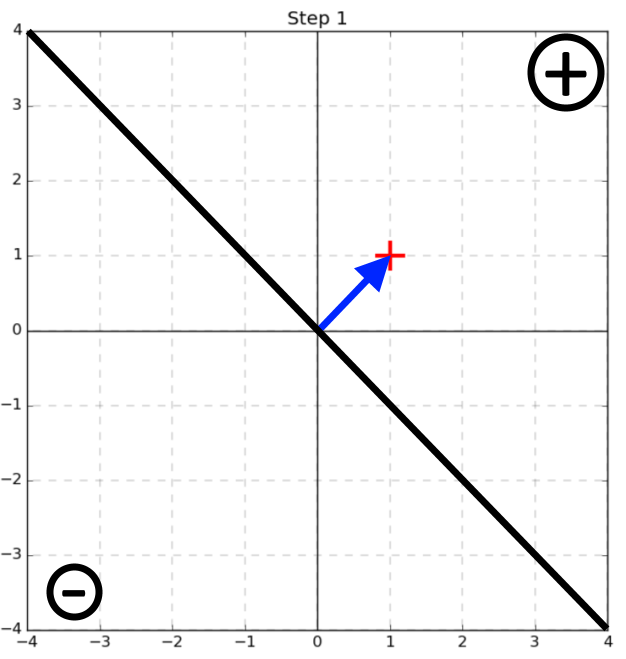
\includegraphics[width=0.24\textwidth]{../Problem_1/step_1.png}}
	\hfill
	\subfloat[Step Two] {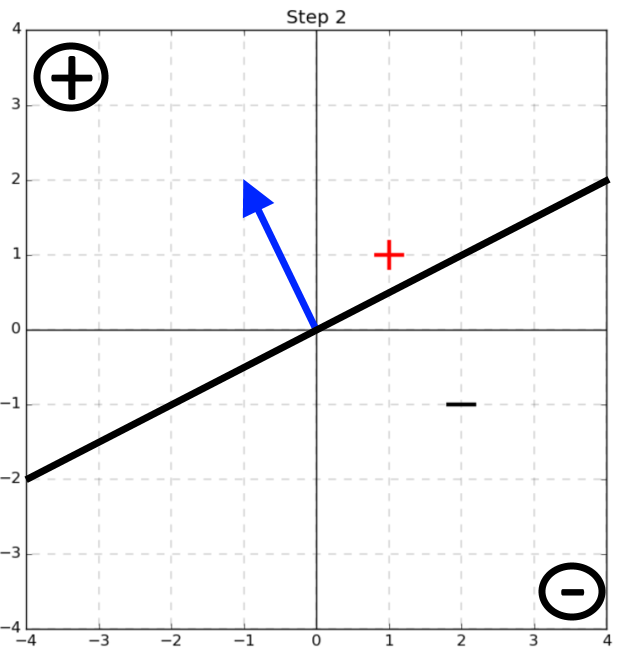
\includegraphics[width=0.24\textwidth]{../Problem_1/step_2.png}}
	\hfill
	\subfloat[Step Three] {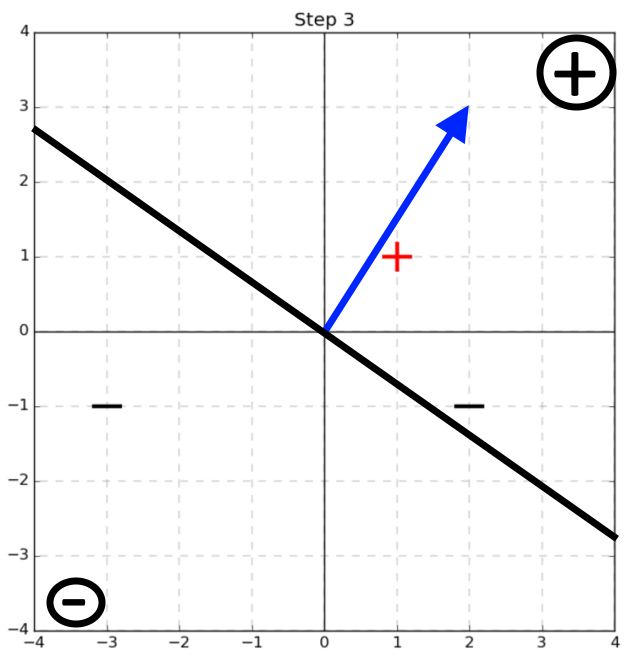
\includegraphics[width=0.24\textwidth]{../Problem_1/step_3.png}}
	\hfill
	\subfloat[Step Four] {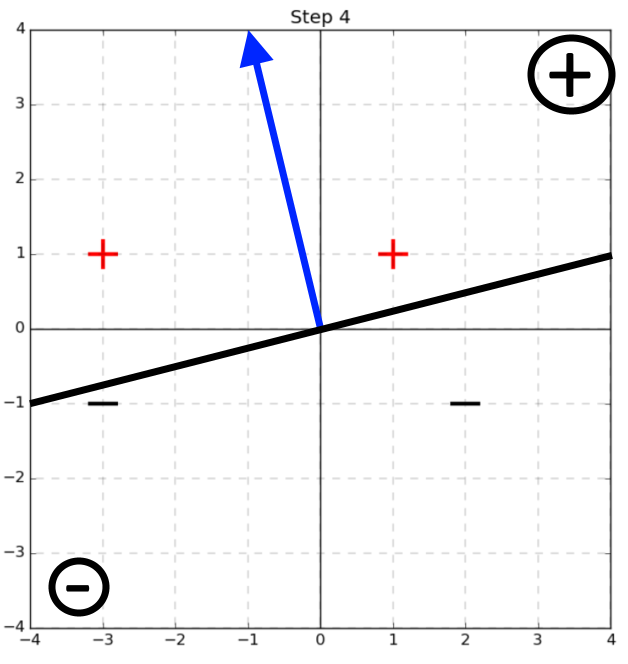
\includegraphics[width=0.24\textwidth]{../Problem_1/step_4.png}}
	\hfill
	\subfloat[Maximum margin] {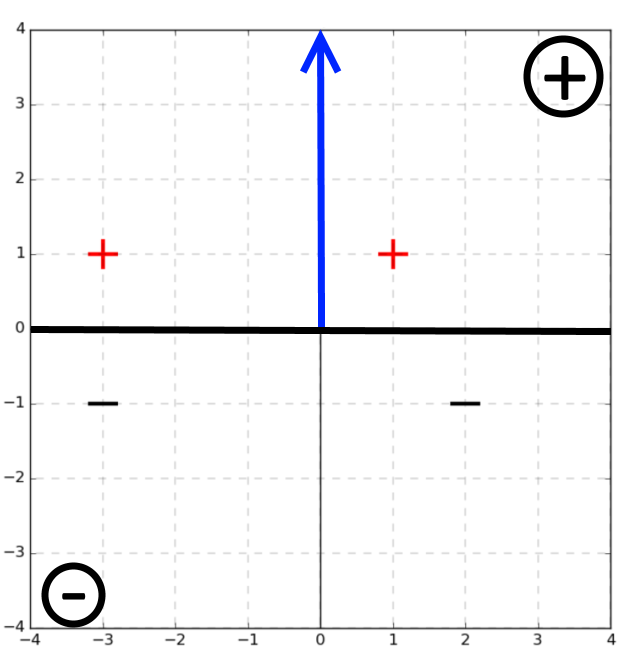
\includegraphics[width=0.24\textwidth]{../Problem_1/opt.png}}
	\caption[]{Visualization of the perceptron's decision boundary. The plots show the weight vector $w$ in blue  and the corresponding decision boundary (black) after they were updated. Plot (e) shows the maximum decision margin which is has the value $1$ in this case. }
	\label{fig:1.1}
\end{figure}
\noindent
To solve Problem 1.3 I will follow the proof according to \cite{CIML}. 
\begin{theorem}
	If data $D$ is linear separable with the geometric margin $\gamma^* = 0.5$ and has the maximum norm $\lVert x \rVert^{2}\leq 5 \forall x \in D$ then the algorithm will convert after at most $\frac{5}{\gamma^2}$ updates. 
\end{theorem}
\begin{proof}
	Suppose $x^*$ realizes $\gamma^*>0$ and let $w^{(k)}$ be the $k^{th}$ weight vector after $k$ updates. We show in the following that the angle between $w$ and $w^*$ decreases such that the algorithm converges. That is when $w^*\cdot w$ increases faster than $\lVert w \rVert^2$.\\
	After the $k^{th}$ update we find
	\begin{align*}
		w^*\cdot w^{(k)} = w^{*}\left( w^{(k-1)}+yx \right) = w*\cdot w^{(k-1)} + yw^*\cdot x \geq w*\cdot w^{(k-1)} + k\gamma 
	\end{align*}
	and
	\begin{align*}
		\lVert w^{(k)} \rVert^2=\lVert w^{(k-1)} + yx \rVert^2 = \lVert w^{(k-1)} \rVert^2 + 2yw^{(k-1)}\cdot x + y^2\cdot\lVert x \rVert^2 \geq \lVert w^{(k-1)} \rVert^2 +5 +0
	\end{align*}
	The last line shows that $\lVert w^{(k)} \rVert$ increases by at least $5$ every update. Therefore $\lVert w^{(k)} \rVert^2 \leq 5k$. So
	\begin{align*}
	\sqrt{5k} \geq \lVert w^{(k)} \rVert \geq w^*\cdot w^{(k)} \geq 5\gamma \Leftrightarrow k \leq \frac{5}{\gamma^2}
	\end{align*}
\end{proof}
\noindent
The maximum number of mistakes (updates) the perceptron has to make until it converges is given by $\frac{5}{\gamma^2}=\frac{5}{0.25}=20$.

\section{Implementation: Perceptron}

% Table generated by Excel2LaTeX from sheet 'Sheet1'
\begin{table}[htbp]
	\centering
	\caption{Add caption}
	\begin{tabularx}{\textwidth}{c|X|X|X|X|}
		& \multicolumn{4}{c|}{question number} \\
		dataset & \multicolumn{1}{c}{2} & \multicolumn{1}{c}{3} & \multicolumn{1}{c}{4} & \multicolumn{1}{c|}{5} \\
		\midrule
		2     &   Is linear separable because error rate doesn't change after $\approx 380$ epochs  &  Does not overfit because testset error doesn't rise     &   No features    & / \\
		\midrule
		3     &   Is linear separable because error rate doesn't change after $\approx 2000$ epochs    &    Does not overfit because testset error doesn't rise   &   No noise    &  \\
		\midrule
		4     &       &       &       &  \\
		\midrule
		5     &       &       &       &  \\
		\midrule
		6     &       &       &       &  \\
		\midrule
		7     &       &       &       &  \\
		\midrule
		8     &       &       &       &  \\
		\midrule
		9     &       &       &       &  \\
		\bottomrule
	\end{tabularx}%
	\label{tab:addlabel}%
\end{table}%



\section{Beat the Perceptron}
 


\section{PCA on Digits}

\subsection{Convariance matrix construction}

Let $X\in \mathbb{R}^{n\times d}$ be the data matrix, $\vec{x}_i \in \mathbb{R}^{d\times 1}$ be the $i^{th}$ element of $X$, $\vec{\mu} \in \mathbb{R}^{d\times 1}$ be the mean vector of all $\vec{x}_i$, $\vec{1}$ be a vector in $\mathbb{R}^{n\times 1}$ consisting of 1's, and $X_c = X - \vec{1}\vec{\mu}^T$ be the centered data matrix. Note that all vectors are considered as column vectors. \par
In figure \ref{fig:4.1.1} ten digits from the MNIST database are plotted, in figure \ref{fig:4.1.3} the mean image ($\vec{\mu}$) is plotted. \par 
 

\begin{figure}[h!]
	\centering
	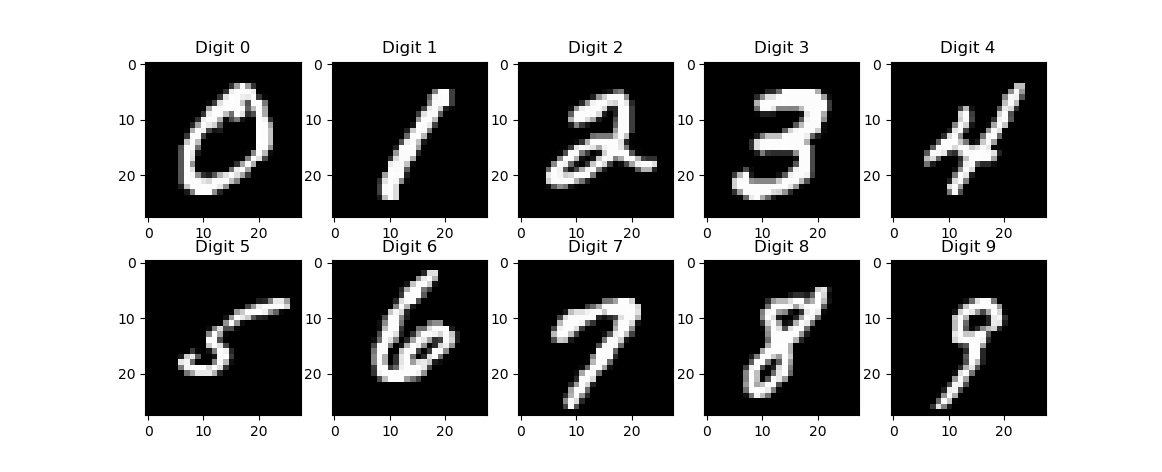
\includegraphics[width=\linewidth]{../Problem_4/Problem_4.1.1.png}
	\caption{Grey scale plot of ten digits of the MNIST database}
	\label{fig:4.1.1}
\end{figure}

\begin{figure}[h!]
	\centering
	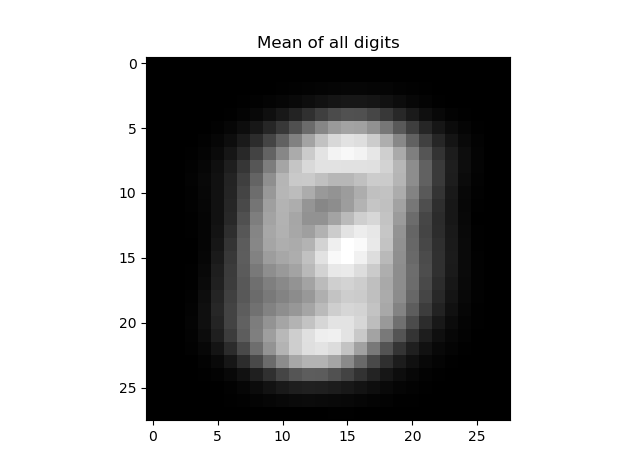
\includegraphics[width=0.66\linewidth]{../Problem_4/Problem_4.1.3_2.png}
	\caption{Grey scale plot of the mean image of the MNIST database}
	\label{fig:4.1.3}
\end{figure}

There are two methods to write down the covariance matrix:
\begin{itemize}
	\item Vector based method:
	\begin{align}
	\Sigma = \frac{1}{n}\sum_{i = 1}^{n} (\vec{x}_i - \vec{\mu})\cdot (\vec{x}_i - \vec{\mu})^T
	\end{align}
	\item Matrix based method:
	\begin{align}
	\Sigma = \frac{1}{n} (X_c^T\cdot X_c)
	\end{align}
\end{itemize}
By considering the dimensions of the centered data matrix $X_c \in \mathbb{R}^{n\times d}$ we find for sigma $\Sigma \in \mathbb{R}^{d\times d}$. \par 
By coding both methods (code attached to .tar.gz, as usual) we found for the vector method a runtime of roughly $191\text{s}$ and $<1$s for the matrix based method. This is in increase of over $19100\%$ in runtime. By testing the average absolute difference between the two methods we found a very small value ($9.78\times 10^{-16}$), in the range of machine precision so the two results are equal.
\textcolor{red}{NUMBER 4.1.6 IS MISSING!}

\subsection{Eigen-Analysis}

By using the SVD on the covariance matrix we find following eigenvalues:
\begin{itemize}
	\item $\lambda_1 = 5.10819064381$
	\item $\lambda_2 = 3.70090586283$
	\item $\lambda_{10} = 1.24026412182$
	\item $\lambda_{30} = 0.362081056419$
	\item $\lambda_{50} = 0.168298737356$
	\item $\sum_{i=1}^{d} \lambda_i = 52.4218857752$
\end{itemize}

The fractional reconstruction error for the first $k=100$ eigenvalues is plotted in figure \ref{fig:4.2.2}.

\begin{figure}
	\centering
	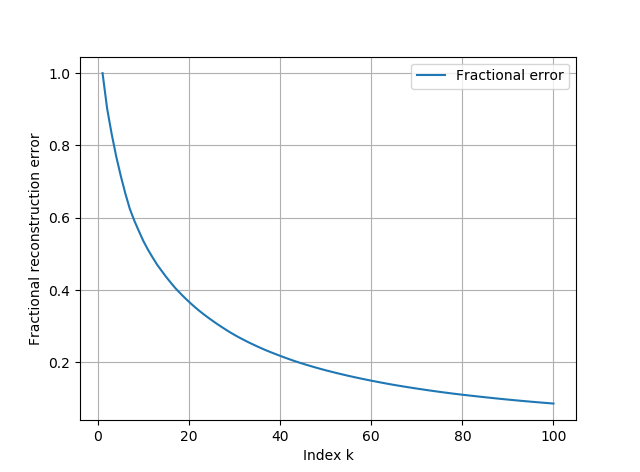
\includegraphics[width=0.66\linewidth]{../Problem_4/Problem_4.2.2.png}
	\caption{Fractional Reconstruction error for the first $k=100$ eigenvalues}
	\label{fig:4.2.2}
\end{figure}

The first $11$ eigenvalues make up $50\%$ of the total variance and the first $44$ eigenvalues make up $80\%$ of the eigenvalues. \par 
The first ten eigenvectors are shown in figure \ref{fig:4.2.4}. They should represent the dimensions with the highest variance (biggest information) and therefore should carry essential information about the ten possible digits, zero to nine.

\begin{figure}
	\centering
	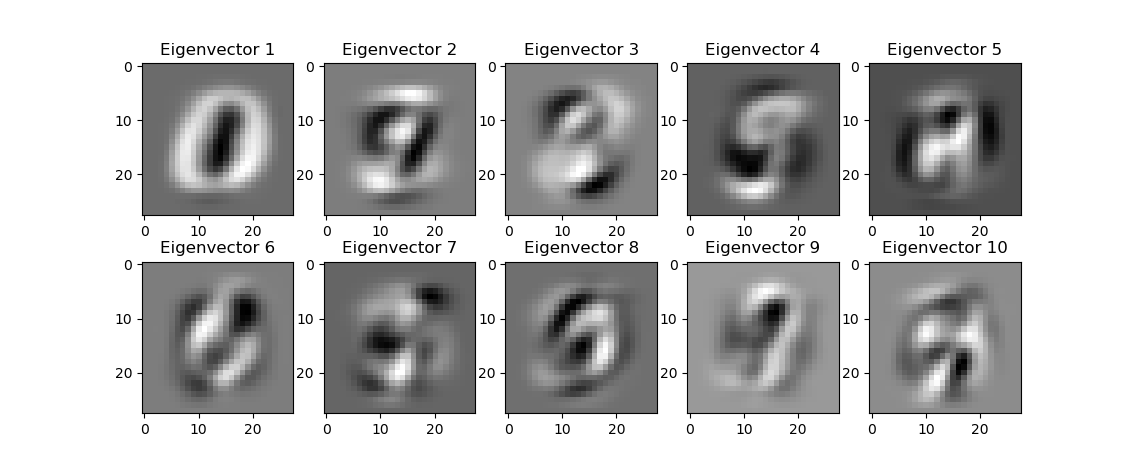
\includegraphics[width=0.66\linewidth]{../Problem_4/Problem_4.2.4.png}
	\caption{Plot of the first ten eigenvectors}
	\label{fig:4.2.4}
\end{figure}

\subsection{Pseudocode for Reconstruction}

Goal: best reconstruction (squared error should be small) for dimensionality reduction from $d$ to $k$ dimensions.
\begin{enumerate}
	\item Use the top $k$ eigenvectors since they carry the larges variance (information) for the reconstruction. The actual number $k$ is a hyperparameter which has to be optimized.
	\item By using SVD on the covariance matrix $\Sigma$ we get the $k$ eigenvalues. The top $k$ eigenvalues make up the matrix $\hat{U}\in \mathbb{R}^{d \times k}$. The reduced data matrix is then given by
	\begin{align}
	\hat{X} = \left( X - \vec{1}\cdot \vec{\mu}^T \right)\cdot \hat{U} 
	\end{align}
	\item The $d$-dimensional reconstruction is then given by
	\begin{align}
	X_\text{rec} = \hat{X}\cdot \hat{U}^T + \vec{1}\cdot\vec{\mu}
	\end{align}
\end{enumerate}

\subsection{Visualization and Reconstruction}

For $k=30$ it takes roughly $2$s to reconstruct the data. The plots are shown for different $k$ in figures \ref{fig:4.4.1} and \ref{fig:4.4.2}. For low values of $k$ ($k=1,3,5$) we can see that the reconstruction is composed of one, three and five eigenvalues. The reconstruction itself is not useful for determining the original digit. For medium $k$ ($k=10,25,50$) the pictures get more and more blurry until for higher $k$ ($k=200,500+$) one finally can estimate the digit.

\begin{figure}[h!]
	\centering
	\subfloat[Reconstruction for $k=1$] {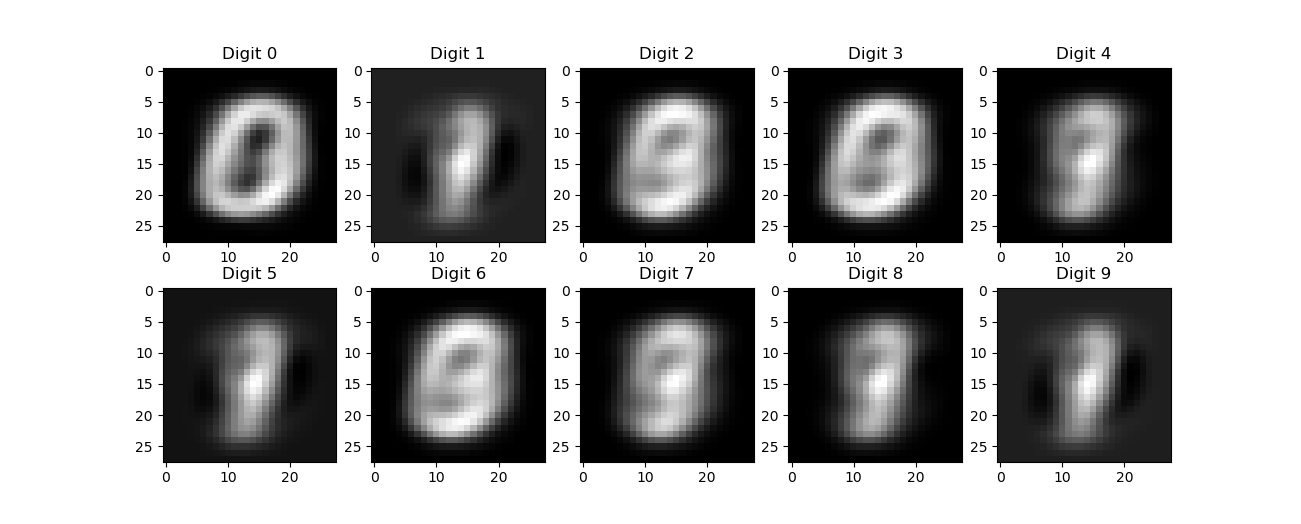
\includegraphics[width=0.88\textwidth]{../Problem_4/Problem_4.4.1.png}}
	\hfill
	\subfloat[Reconstruction for $k=3$] {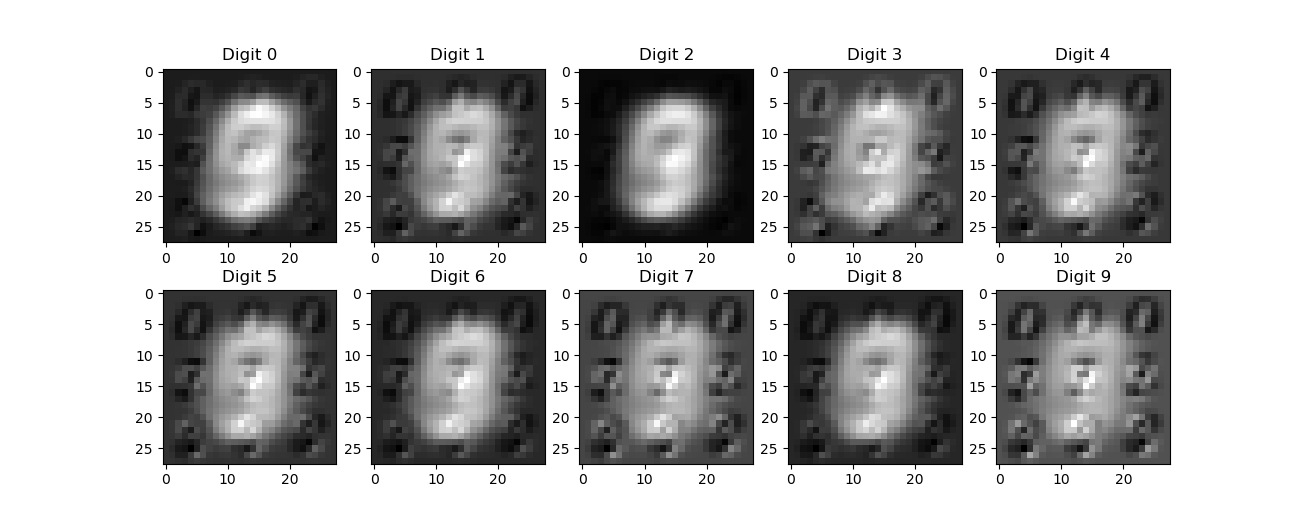
\includegraphics[width=0.88\textwidth]{../Problem_4/Problem_4.4.3.png}}
	\hfill
	\subfloat[Reconstruction for $k=5$] {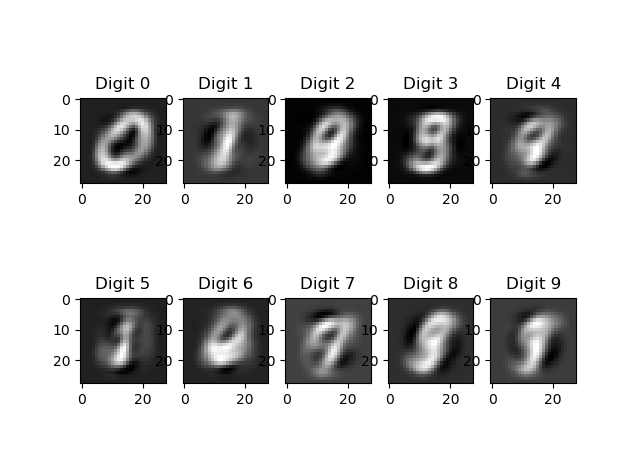
\includegraphics[width=0.88\textwidth]{../Problem_4/Problem_4.4.5.png}}
	\hfill
	\subfloat[Reconstruction for $k=10$] {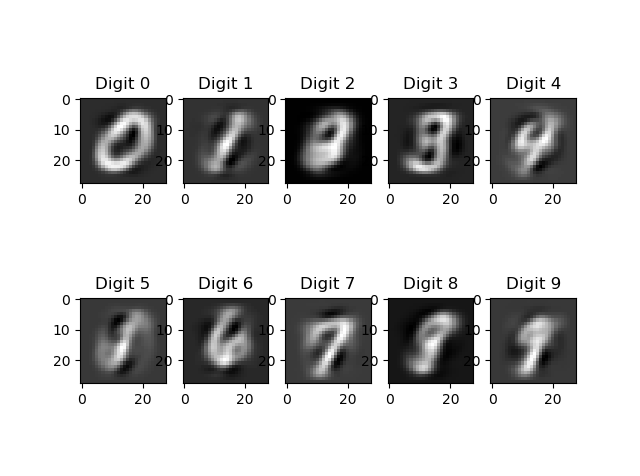
\includegraphics[width=0.88\textwidth]{../Problem_4/Problem_4.4.10.png}}
	\caption[]{Reconstruction of the ten digits used in Problem part 4.1 for different $k$.}
	\label{fig:4.4.1}
\end{figure}
\begin{figure}[h!]
	\centering
	\subfloat[Reconstruction for $k=25$] {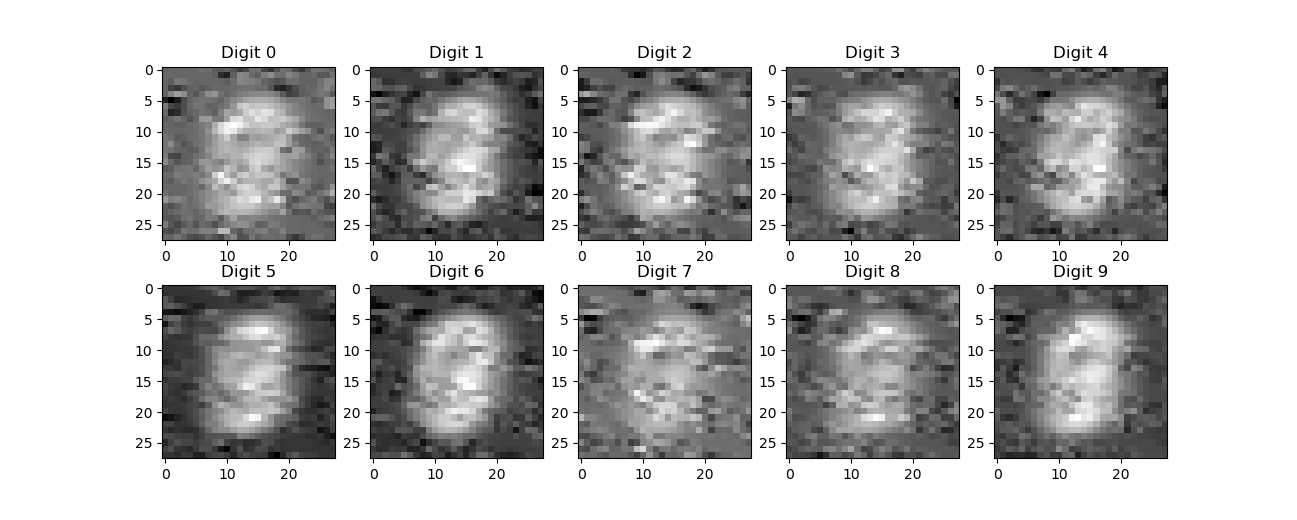
\includegraphics[width=0.88\textwidth]{../Problem_4/Problem_4.4.25.png}}
	\hfill
	\subfloat[Reconstruction for $k=50$] {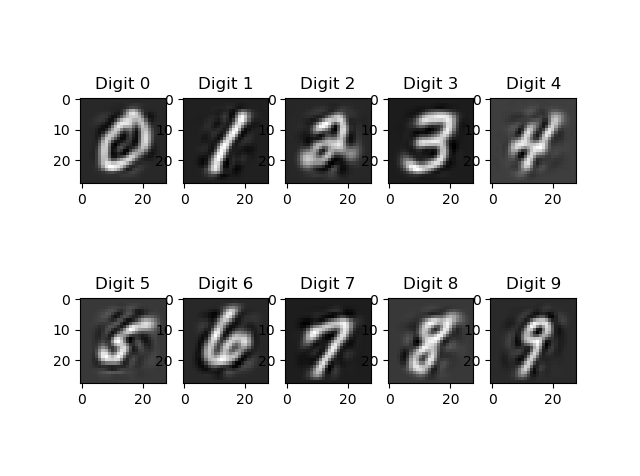
\includegraphics[width=0.88\textwidth]{../Problem_4/Problem_4.4.50.png}}
	\hfill
	\subfloat[Reconstruction for $k=200$] {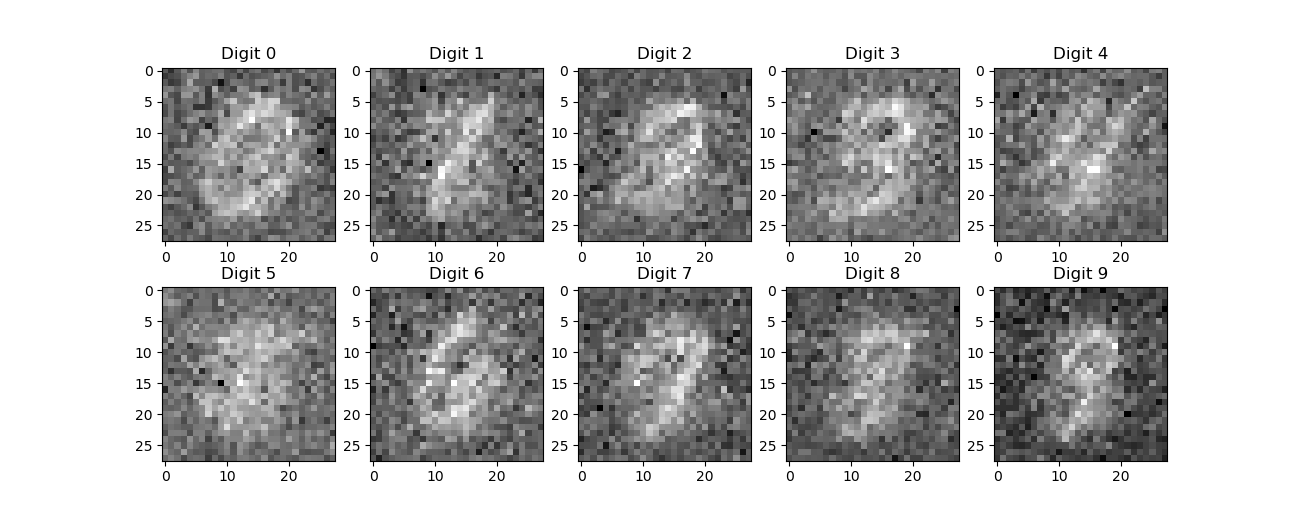
\includegraphics[width=0.88\textwidth]{../Problem_4/Problem_4.4.200.png}}
	\hfill
	\subfloat[Reconstruction for $k=500$] {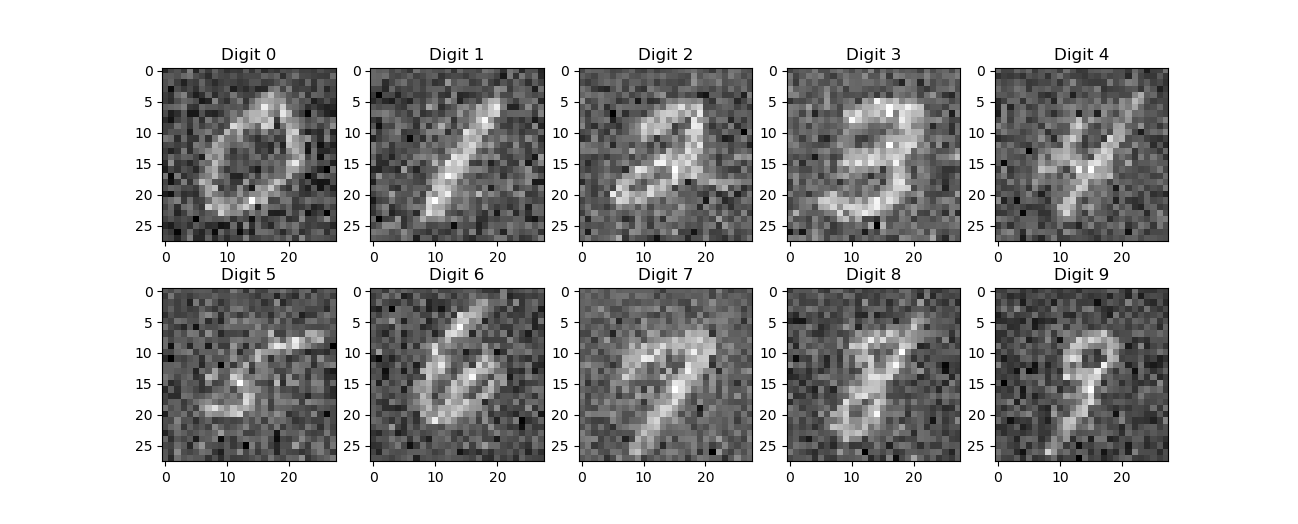
\includegraphics[width=0.88\textwidth]{../Problem_4/Problem_4.4.500.png}}
	\caption[]{Reconstruction of the ten digits used in Problem part 4.1 for different $k$. Continuation from previous page.}
	\label{fig:4.4.2}
\end{figure}





\section{Bayes Optimal Classifier}



\section{Bonus: Dimensionality Reduction}


\section{Bonus: The Bayes Optimal Hypothesis for Regression}


\chapter*{Bibliography}
\addcontentsline{toc}{chapter}{Bibliography}%	

\bibliographystyle{unsrt}
\bibliography{./bib}





\end{document}  